
\documentclass[10pt,journal,onecolumn]{IEEEtran}
\usepackage[utf8]{inputenc}
\usepackage[T1]{fontenc}
\usepackage{hyperref}
\usepackage{longtable}
\usepackage{array}
\usepackage{booktabs}
\usepackage{enumitem}
\usepackage{tikz}
\usetikzlibrary{arrows.meta,positioning,shapes.geometric,fit}
\usepackage{geometry}
\geometry{margin=0.75in}
\hypersetup{hidelinks}
\newcolumntype{P}[1]{>{\raggedright\arraybackslash}p{#1}}
\title{JMCP and JPCM: A Final Protocol-First Architecture for Sovereign Agent Control, Evidence, Task Management, Tool Awareness, Voice Interaction, and Self-Improving Software Operations}
\author{Jepson Taylor Design Study -- Final V5 Hardened Specification}
\begin{document}
\maketitle
\begin{abstract}
The Joint Master Control Plane (JMCP) is proposed as a sovereign control plane for agentic software operations. Its protocol, Joint Process/Control Messaging (JPCM), is defined as the mandatory communication standard for all services, tools, agents, data stores, user interfaces, voice interfaces, and self-improvement pipelines. The core claim is that high-value autonomy requires more than tool calling, multi-agent routing, observability, or workflow automation. It requires signed authority, scoped capability leases, evidence-bound task state, attention governance, replayable causality, and quarantined learning. This paper criticizes the preceding V4 artifacts, identifies residual failure modes, and presents a final protocol-first architecture that can manage ordinary tasks, incidents, code changes, research, knowledge compression, automated tool building, and self-modification while preserving human authority. The design is intentionally ambitious: JMCP is positioned as a fab-style process-control and fault-detection layer for knowledge work, where the human remains above the noise and the control plane governs the machines below.
\end{abstract}
\begin{IEEEkeywords}
agent control plane, model context protocol, agent-to-agent protocol, observability, autonomous software engineering, AI safety, capability leases, evidence ledger, voice interface, self-improvement, tool building.
\end{IEEEkeywords}

\section{Introduction}
Software organizations are rapidly gaining access to coding agents, tool protocols, retrieval systems, CI automation, workflow engines, and voice/text assistants. These systems increase surface area but not necessarily control. A repository can be modified by a coding agent, a ticket can be summarized by a model, a tool can be exposed by a protocol server, and a dashboard can show traces; yet no single layer may know which action is authorized, which evidence is real, which task owns a change, which user decision is required, or whether a lesson should become durable policy. JMCP addresses that gap.

The final thesis is precise. JMCP is the authority and evidence control plane. JPCM is the wire-level law all services must speak. Agents are workers, not authorities. Tools are capabilities, not permissions. Logs are raw material, not proof. Memory is quarantined until promoted. Voice is a command modality only when bounded by confidence and confirmation. Self-improvement is possible only through staged evidence.

\section{Critique of the V4 Inputs}
\begin{longtable}{P{0.32\textwidth} P{0.08\textwidth} P{0.55\textwidth}}
\toprule
Artifact & Score & Principal critique \\
\midrule
JMCP\_V4\_ENGINEERING\_SPEC.md & 86 & Strong architecture and evidence posture, but protocol obligations are still partially narrative and not enough negative conformance tests exist. \\
JMCP\_V4\_engineering\_spec(1).md & 88 & Better operational detail and task flow, but still needs a fully normative wire schema and service-card negotiation rules. \\
JMCP\_V4\_ieee\_whitepaper.tex & 85 & Clear paper structure, but insufficient page-level depth on protocol compatibility and formal task semantics. \\
jmcp\_cp\_v1\_envelope.schema.json & 63 & Useful seed envelope, but too small for final use: it lacks full payload taxonomy, service cards, user-attention contract, leases, and task semantics. \\
jmcp\_v4\_ieee\_white\_paper.tex & 88 & Mature paper with good related work; needs stronger diagrams, more references, and clearer falsifiable claims. \\
jmcp\_v4\_jpcp\_v1\_envelope\_schema.json & 64 & Slightly broader seed schema, but still not a complete service protocol or validation surface. \\
jmcp\_v4\_protocol\_first\_engineering\_spec(1).md & 87 & Good control-plane framing, but user-attention, voice, and offline/degraded modes remain under-specified. \\
jmcp\_v4\_protocol\_first\_engineering\_spec.md & 90 & Best V4 spec: protocol-first framing is right. Remaining gap: task leases, context budgets, and automated tool building need explicit schemas. \\
jmcp\_v4\_protocol\_first\_ieee\_paper.tex & 90 & Strongest paper input; protocol-first argument is persuasive, but still short of a complete standard and full conformance suite. \\
jmcp\_v4\_scorecard.md & 82 & Useful critique, but the scorecard is not adversarial enough about false evidence, governance capture, and recursive self-improvement failures. \\
jmcp\_v4\_whitepaper.tex & 87 & Ambitious and readable, but it blends system vision and implementation details without enough normative separation. \\
\bottomrule
\end{longtable}

The V4 generation was directionally strong because it made protocol finality central. It still left three concerns insufficiently final. First, the protocol envelope existed but did not fully cover service cards, user attention, self-improvement, automated tool building, and voice as first-class payloads. Second, task state and evidence were described, but not made sufficiently replayable and hostile-testable. Third, the future vector remained ambitious but did not define the required controls for a system that can build new tools and improve itself.

\section{Related Work and Boundary}
MCP standardizes application-to-tool and application-to-context integration; A2A standardizes agent discovery, tasks, artifacts, and inter-agent communication. JMCP does not replace these systems. It supervises them through JPCM adapters. Observability systems such as OpenTelemetry describe traces, metrics, and logs; JMCP treats those signals as evidence candidates that must be bound to tasks, claims, and authority decisions. CloudEvents and AsyncAPI influence event shape and stream design, but they do not define agent authority, attention budgets, or self-improvement quarantine. Security frameworks such as OWASP LLM Top 10, NIST AI RMF, SLSA, Sigstore, in-toto, and CycloneDX inform controls for prompt injection, excessive agency, provenance, and supply-chain integrity. JMCP combines these concerns into a protocol-driven control plane.

\section{System Definition}
JMCP is not a universal agent, not a dashboard, not a workflow engine, and not a tool registry. It is a control system. It observes the world, reasons about tasks, grants leases, collects evidence, manages attention, learns cautiously, and delegates execution to constrained services. It is analogous to a fab-level process-control and fault-detection system for knowledge work: it monitors equipment, detects drift, prevents unsafe operations, and escalates only what humans must decide.

\begin{figure}[h]
\centering
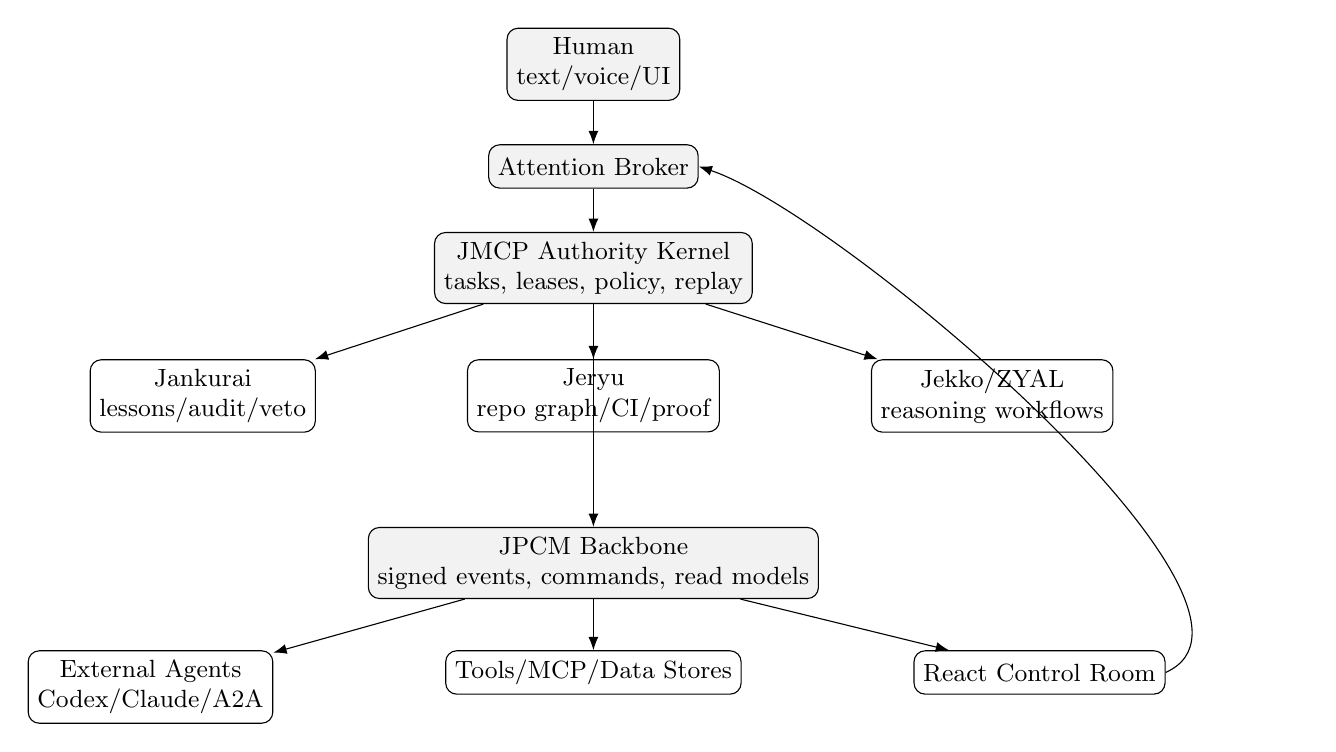
\begin{tikzpicture}[node distance=0.55cm, every node/.style={font=\small}, box/.style={draw, rounded corners, align=center, minimum height=0.55cm}, arr/.style={-Latex}]
\node[box, fill=gray!10] (user) {Human\\text/voice/UI};
\node[box, below=of user, fill=gray!10] (attn) {Attention Broker};
\node[box, below=of attn, fill=gray!10] (jmcp) {JMCP Authority Kernel\\tasks, leases, policy, replay};
\node[box, below left=0.7cm and 1.5cm of jmcp] (jankurai) {Jankurai\\lessons/audit/veto};
\node[box, below=0.7cm of jmcp] (jeryu) {Jeryu\\repo graph/CI/proof};
\node[box, below right=0.7cm and 1.5cm of jmcp] (jekko) {Jekko/ZYAL\\reasoning workflows};
\node[box, below=1.2cm of jeryu, fill=gray!10] (bus) {JPCM Backbone\\signed events, commands, read models};
\node[box, below left=0.65cm and 1.2cm of bus] (agents) {External Agents\\Codex/Claude/A2A};
\node[box, below=0.65cm of bus] (tools) {Tools/MCP/Data Stores};
\node[box, below right=0.65cm and 1.2cm of bus] (ui) {React Control Room};
\draw[arr] (user)--(attn); \draw[arr] (attn)--(jmcp); \draw[arr] (jmcp)--(jankurai); \draw[arr] (jmcp)--(jeryu); \draw[arr] (jmcp)--(jekko); \draw[arr] (jmcp)--(bus); \draw[arr] (bus)--(agents); \draw[arr] (bus)--(tools); \draw[arr] (bus)--(ui); \draw[arr] (ui.east) .. controls +(1.8,0.8) and +(1.8,-0.6) .. (attn.east);
\end{tikzpicture}
\caption{JMCP is the authority and evidence layer; JPCM is the communication backbone.}
\end{figure}

\section{JPCM 1.0.0 Normative Envelope}
Every message is a signed envelope with schema version, envelope identifier, event type, event time, producer, authority context, task reference, routing, context contract, payload, evidence, observability, attention, privacy, and integrity. Unknown extension fields are allowed only under an extension namespace and cannot change authority semantics. The canonical schema is delivered as \texttt{JPCM\_FINAL\_PROTOCOL\_SCHEMA\_v1.0.0.json}.

\subsection{Event Families}
The required event families are service card, health, capability lease, task lifecycle, tool invocation, data query, evidence, user message, voice, policy lesson, self-improvement, tool build, incident, and disaster mode. A service that cannot express its behavior within these families is non-conformant or must be wrapped by an adapter.

\subsection{Effect Classes}
Effect classes range from observation to production deployment, policy change, authority change, self-modification, tool creation, secret access, and external spending. Each effect class has a minimum approval and evidence standard. High-effect classes require human approval or a preauthorized policy, signed leases, and replayable evidence.

\section{Task Semantics}
All work is represented as a task. Tasks can be user-originated or autonomous, synchronous or background, strategic or tactical. The lifecycle is shown in Fig.~\ref{fig:task}.

\begin{figure}[h]
\centering
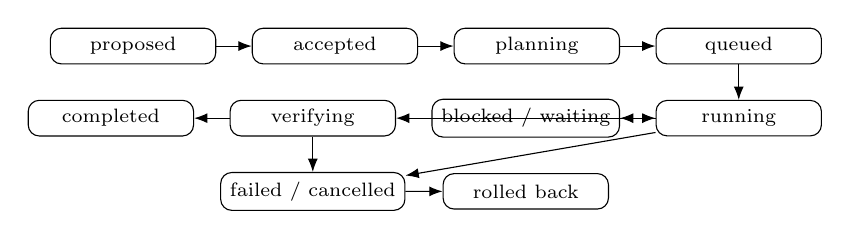
\begin{tikzpicture}[node distance=0.45cm, every node/.style={font=\scriptsize}, st/.style={draw, rounded corners, align=center, minimum width=2.1cm, minimum height=0.45cm}, arr/.style={-Latex}]
\node[st] (p) {proposed};
\node[st, right=of p] (a) {accepted};
\node[st, right=of a] (pl) {planning};
\node[st, right=of pl] (q) {queued};
\node[st, below=of q] (r) {running};
\node[st, left=of r] (b) {blocked / waiting};
\node[st, left=of b] (v) {verifying};
\node[st, left=of v] (c) {completed};
\node[st, below=of v] (f) {failed / cancelled};
\node[st, below=of b] (rb) {rolled back};
\draw[arr] (p)--(a); \draw[arr] (a)--(pl); \draw[arr] (pl)--(q); \draw[arr] (q)--(r); \draw[arr] (r)--(b); \draw[arr] (b)--(r); \draw[arr] (r)--(v); \draw[arr] (v)--(c); \draw[arr] (r)--(f); \draw[arr] (v)--(f); \draw[arr] (f)--(rb);
\end{tikzpicture}
\caption{Canonical JPCM task lifecycle.}
\label{fig:task}
\end{figure}

A task is not complete because an agent says it is complete. It is complete when its success criteria are satisfied by evidence, its effect class obligations are met, and the authority kernel records a signed state transition.

\section{Communication Backbone}
The communication backbone has command, event, and read-model planes. Commands are lease-checked and fail closed. Events are append-only and signed. Read models are optimized for the control room and may lag, but must display freshness. Priority lanes separate real-time voice and incidents from normal background work and bulk analysis. Replay reconstructs the system state from the event log and evidence ledger.

\begin{figure}[h]
\centering
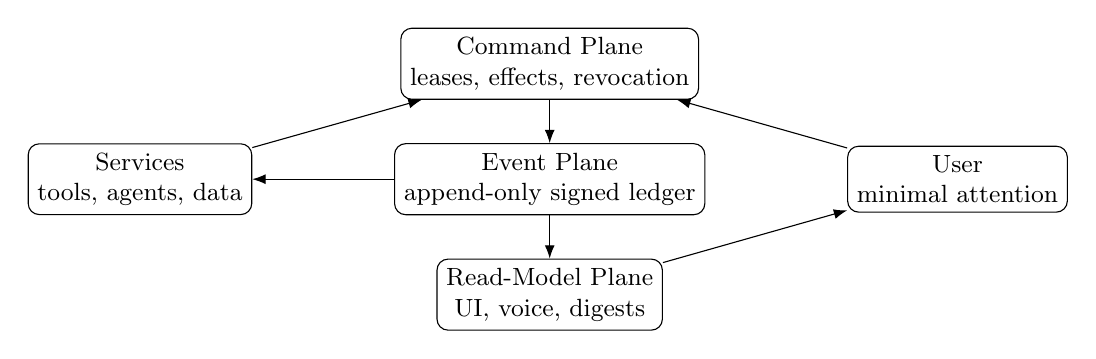
\begin{tikzpicture}[node distance=0.55cm, every node/.style={font=\small}, box/.style={draw, rounded corners, align=center, minimum height=0.55cm}, arr/.style={-Latex}]
\node[box] (cmd) {Command Plane\\leases, effects, revocation};
\node[box, below=of cmd] (evt) {Event Plane\\append-only signed ledger};
\node[box, below=of evt] (read) {Read-Model Plane\\UI, voice, digests};
\node[box, left=1.8cm of evt] (services) {Services\\tools, agents, data};
\node[box, right=1.8cm of evt] (user) {User\\minimal attention};
\draw[arr] (services)--(cmd); \draw[arr] (cmd)--(evt); \draw[arr] (evt)--(read); \draw[arr] (read)--(user); \draw[arr] (user)--(cmd); \draw[arr] (evt)--(services);
\end{tikzpicture}
\caption{The backbone separates authority-changing commands from replayable events and fast read models.}
\end{figure}

\section{Attention Governance}
The user's attention is a protected resource. JMCP must avoid both flooding and under-escalation. The attention broker classifies each event as none, digest, decision, urgent, incident, or voice confirmation. The default should be non-interruption. The exception is high-effect, high-uncertainty, irreversible, user-preference-sensitive, or incident-related work. The user must be able to drill down from a minimal summary to task, evidence, trace, raw artifact, and policy decision.

\section{Voice and Text Interaction}
Voice is a first-class channel but not an ambient authority channel. High-effect voice requests require speaker/session binding, transcript confidence, intent classification, readback, and explicit confirmation. The protocol records voice turns, transcripts, confidence, confirmation state, and audio evidence references. Text and UI messages use the same task and attention semantics.

\section{Tool and Data Awareness}
JMCP maintains a live capability map. It knows the tools available, what effect classes they support, their costs, their known failure modes, their data surfaces, their conformance level, and their usage history. It also knows data stores, data classes, freshness, owners, sensitivity, and schema. This map drives routing decisions and tool-building proposals.

\section{Automated Tool Building}
A mature JMCP does not only use tools; it decides when a new tool should exist. Automated tool building is governed by reuse search, capability-gap proof, sandboxed implementation, SBOM, provenance, malicious-input testing, benchmark evaluation, canary promotion, and deprecation rules. Generated tools are never admitted directly into trusted production capability maps.

\section{Self-Improvement}
Self-improvement is the most dangerous and most valuable task family. It includes changes to prompts, routing, policies, schemas, memory, tools, models, UI, and code. The promotion ladder is proposal, quarantine, shadow, canary, staging, production, and periodic revalidation. Authority-changing modifications require human approval and rollback plans.

\begin{figure}[h]
\centering
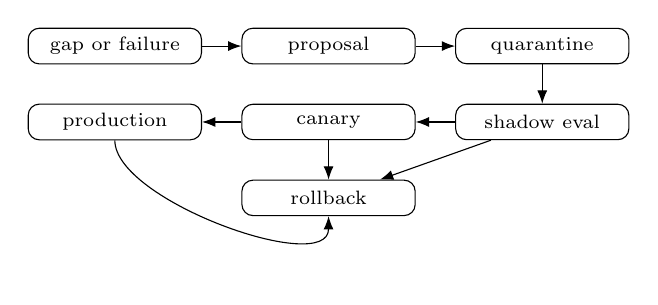
\begin{tikzpicture}[node distance=0.5cm, every node/.style={font=\scriptsize}, st/.style={draw, rounded corners, align=center, minimum width=2.2cm, minimum height=0.45cm}, arr/.style={-Latex}]
\node[st] (g) {gap or failure};
\node[st, right=of g] (prop) {proposal};
\node[st, right=of prop] (q) {quarantine};
\node[st, below=of q] (shadow) {shadow eval};
\node[st, left=of shadow] (canary) {canary};
\node[st, left=of canary] (prod) {production};
\node[st, below=of canary] (roll) {rollback};
\draw[arr] (g)--(prop); \draw[arr] (prop)--(q); \draw[arr] (q)--(shadow); \draw[arr] (shadow)--(canary); \draw[arr] (canary)--(prod); \draw[arr] (shadow)--(roll); \draw[arr] (canary)--(roll); \draw[arr] (prod) .. controls +(0,-1.0) and +(0,-1.0) .. (roll);
\end{tikzpicture}
\caption{Self-improvement and automated tool building use staged promotion and rollback.}
\end{figure}

\section{Security Model}
The security model assumes prompt injection, malicious repos, malicious tools, lying agents, stale evidence, compromised dependencies, overbroad permissions, user fatigue, and partial outages. Controls include service identity, signed envelopes, least-privilege leases, sandboxing, network egress policy, content-addressed evidence, task replay, secret redaction, and supply-chain attestations.

\section{Failure-Mode Analysis}
\begin{longtable}{P{0.04\textwidth} P{0.18\textwidth} P{0.35\textwidth} P{0.35\textwidth}}
\toprule
\# & Failure & Scenario & Control \\
\midrule
1 & Protocol drift & Services quietly add non-standard fields or bypass leases & Schema validation, signed conformance receipts, reject unknown required semantics \\
2 & Authority confusion & Agents treat advice as approval or confuse advisory and execution channels & Effect classes, explicit approval state, enforcement at runner and bus \\
3 & False evidence & Logs, test results, or screenshots are fabricated or stale & Content-addressed evidence, verifier identity, replayable commands, quorum checks \\
4 & Context poisoning & Untrusted repo docs or web pages inject instructions into task memory & Source taint labels, role separation, context firewall, quoted untrusted material \\
5 & Lease overbreadth & A worker receives more permission than task needs & Least-privilege lease compiler and expiring scoped tokens \\
6 & Recursive self-modification & JMCP improves itself into a broken or unsafe state & Shadow mode, canary rollout, quarantine, rollback, human approval for authority changes \\
7 & User-attention flooding & Everything becomes an escalation and the user stops trusting it & Attention budgets, severity thresholds, digesting, decision bundling \\
8 & User under-involvement & The system hides a critical decision or irreversible effect & Mandatory human gates for high-effect classes and unknown risk \\
9 & Voice ambiguity & Speech recognition turns a casual statement into an action & Confirm high-effect actions, voice intent confidence, readback, session binding \\
10 & Backbone overload & Telemetry volume swamps the control plane & Tiered streams, sampling, priority lanes, backpressure, local buffering \\
11 & Split brain & Multiple JMCP instances issue conflicting decisions & Consensus lease holder, epoch fencing, monotonic sequence numbers \\
12 & Data exfiltration & Agents leak secrets through prompts, logs, traces, or external tools & Secret scanners, egress policy, redaction, data-classified leases \\
13 & Supply-chain compromise & Tool dependency or generated tool is malicious & SBOM, SLSA provenance, signatures, sandboxed build, reproducible checks \\
14 & Policy capture & A bad lesson becomes global law and blocks good work & Jankurai lesson quarantine, challenge/appeal process, expiry and confidence \\
15 & Observability theater & Dashboards look complete but omit causal proof & Evidence graph, trace-task correlation, missing-evidence alerts \\
16 & Planner hallucination & JMCP scopes impossible work with confident estimates & Capability registry, cost model, dry-run, feasibility probes \\
17 & Adversarial repo & Malicious code exploits analysis or build tools & Hermetic sandbox, read-only mounts, network denial, resource caps \\
18 & Tool sprawl & The system builds many overlapping tools & Tool inventory, reuse scoring, deprecation, capability map \\
19 & Semantic mismatch & MCP/A2A/OpenAPI tools report success using incompatible meanings & Adapters translate into JPCM effects and evidence taxonomy \\
20 & Stale knowledge graph & Jeryu graph lags behind actual code & Freshness stamps, invalidation on commit, stale-source penalties \\
21 & Runaway optimization & JMCP optimizes metrics while harming user goals & Goal charter, user-value KPIs, periodic alignment review \\
22 & Silent degraded mode & Components fail but UI still presents confident status & Health leases, degraded-state badges, fail-closed for high effects \\
23 & Temporal inconsistency & Tasks rely on outdated policy, schema, or repo state & Version pinning, schema epochs, rebasing checkpoints \\
24 & Cross-tenant bleed & Lessons/data from one tenant contaminate another & Tenant isolation, anonymized promotion pipeline, access proofs \\
25 & Unsafe automation & Automation outruns review and deploys broken code & Promotion ladder, staged effects, CI veto, Jankurai proof gate \\
26 & Ambiguous ownership & No service owns a decision, artifact, or incident & Every event has responsible authority and owner service \\
27 & Inadequate incident reconstruction & After failure, causality cannot be rebuilt & Append-only event log, causal IDs, evidence bundles, retention policy \\
28 & Prompt/tool identity spoofing & A malicious service pretends to be a trusted one & mTLS, JWS signatures, service-card registry, key rotation \\
29 & Schema ossification & Protocol cannot evolve without breaking services & Semver, capability negotiation, extension namespaces, deprecation windows \\
30 & Over-centralization & JMCP becomes a bottleneck or single point of failure & Control/read-plane separation, local autonomous execution, replicated read models \\
\bottomrule
\end{longtable}

\section{Conformance Test Suite}
\begin{longtable}{P{0.05\textwidth} P{0.16\textwidth} P{0.38\textwidth} P{0.33\textwidth}}
\toprule
\# & Area & Test & Expected result \\
\midrule
1 & signature & Inject malformed or adversarial signature condition 1 & JMCP rejects, quarantines, or escalates with a signed reason and replayable evidence \\
2 & lease & Inject malformed or adversarial lease condition 2 & JMCP rejects, quarantines, or escalates with a signed reason and replayable evidence \\
3 & task & Inject malformed or adversarial task condition 3 & JMCP rejects, quarantines, or escalates with a signed reason and replayable evidence \\
4 & evidence & Inject malformed or adversarial evidence condition 4 & JMCP rejects, quarantines, or escalates with a signed reason and replayable evidence \\
5 & attention & Inject malformed or adversarial attention condition 5 & JMCP rejects, quarantines, or escalates with a signed reason and replayable evidence \\
6 & voice & Inject malformed or adversarial voice condition 6 & JMCP rejects, quarantines, or escalates with a signed reason and replayable evidence \\
7 & self-improvement & Inject malformed or adversarial self-improvement condition 7 & JMCP rejects, quarantines, or escalates with a signed reason and replayable evidence \\
8 & tool-build & Inject malformed or adversarial tool-build condition 8 & JMCP rejects, quarantines, or escalates with a signed reason and replayable evidence \\
9 & replay & Inject malformed or adversarial replay condition 9 & JMCP rejects, quarantines, or escalates with a signed reason and replayable evidence \\
10 & schema & Inject malformed or adversarial schema condition 10 & JMCP rejects, quarantines, or escalates with a signed reason and replayable evidence \\
11 & signature & Inject malformed or adversarial signature condition 11 & JMCP rejects, quarantines, or escalates with a signed reason and replayable evidence \\
12 & lease & Inject malformed or adversarial lease condition 12 & JMCP rejects, quarantines, or escalates with a signed reason and replayable evidence \\
13 & task & Inject malformed or adversarial task condition 13 & JMCP rejects, quarantines, or escalates with a signed reason and replayable evidence \\
14 & evidence & Inject malformed or adversarial evidence condition 14 & JMCP rejects, quarantines, or escalates with a signed reason and replayable evidence \\
15 & attention & Inject malformed or adversarial attention condition 15 & JMCP rejects, quarantines, or escalates with a signed reason and replayable evidence \\
16 & voice & Inject malformed or adversarial voice condition 16 & JMCP rejects, quarantines, or escalates with a signed reason and replayable evidence \\
17 & self-improvement & Inject malformed or adversarial self-improvement condition 17 & JMCP rejects, quarantines, or escalates with a signed reason and replayable evidence \\
18 & tool-build & Inject malformed or adversarial tool-build condition 18 & JMCP rejects, quarantines, or escalates with a signed reason and replayable evidence \\
19 & replay & Inject malformed or adversarial replay condition 19 & JMCP rejects, quarantines, or escalates with a signed reason and replayable evidence \\
20 & schema & Inject malformed or adversarial schema condition 20 & JMCP rejects, quarantines, or escalates with a signed reason and replayable evidence \\
21 & signature & Inject malformed or adversarial signature condition 21 & JMCP rejects, quarantines, or escalates with a signed reason and replayable evidence \\
22 & lease & Inject malformed or adversarial lease condition 22 & JMCP rejects, quarantines, or escalates with a signed reason and replayable evidence \\
23 & task & Inject malformed or adversarial task condition 23 & JMCP rejects, quarantines, or escalates with a signed reason and replayable evidence \\
24 & evidence & Inject malformed or adversarial evidence condition 24 & JMCP rejects, quarantines, or escalates with a signed reason and replayable evidence \\
25 & attention & Inject malformed or adversarial attention condition 25 & JMCP rejects, quarantines, or escalates with a signed reason and replayable evidence \\
26 & voice & Inject malformed or adversarial voice condition 26 & JMCP rejects, quarantines, or escalates with a signed reason and replayable evidence \\
27 & self-improvement & Inject malformed or adversarial self-improvement condition 27 & JMCP rejects, quarantines, or escalates with a signed reason and replayable evidence \\
28 & tool-build & Inject malformed or adversarial tool-build condition 28 & JMCP rejects, quarantines, or escalates with a signed reason and replayable evidence \\
29 & replay & Inject malformed or adversarial replay condition 29 & JMCP rejects, quarantines, or escalates with a signed reason and replayable evidence \\
30 & schema & Inject malformed or adversarial schema condition 30 & JMCP rejects, quarantines, or escalates with a signed reason and replayable evidence \\
31 & signature & Inject malformed or adversarial signature condition 31 & JMCP rejects, quarantines, or escalates with a signed reason and replayable evidence \\
32 & lease & Inject malformed or adversarial lease condition 32 & JMCP rejects, quarantines, or escalates with a signed reason and replayable evidence \\
33 & task & Inject malformed or adversarial task condition 33 & JMCP rejects, quarantines, or escalates with a signed reason and replayable evidence \\
34 & evidence & Inject malformed or adversarial evidence condition 34 & JMCP rejects, quarantines, or escalates with a signed reason and replayable evidence \\
35 & attention & Inject malformed or adversarial attention condition 35 & JMCP rejects, quarantines, or escalates with a signed reason and replayable evidence \\
36 & voice & Inject malformed or adversarial voice condition 36 & JMCP rejects, quarantines, or escalates with a signed reason and replayable evidence \\
37 & self-improvement & Inject malformed or adversarial self-improvement condition 37 & JMCP rejects, quarantines, or escalates with a signed reason and replayable evidence \\
38 & tool-build & Inject malformed or adversarial tool-build condition 38 & JMCP rejects, quarantines, or escalates with a signed reason and replayable evidence \\
39 & replay & Inject malformed or adversarial replay condition 39 & JMCP rejects, quarantines, or escalates with a signed reason and replayable evidence \\
40 & schema & Inject malformed or adversarial schema condition 40 & JMCP rejects, quarantines, or escalates with a signed reason and replayable evidence \\
41 & signature & Inject malformed or adversarial signature condition 41 & JMCP rejects, quarantines, or escalates with a signed reason and replayable evidence \\
42 & lease & Inject malformed or adversarial lease condition 42 & JMCP rejects, quarantines, or escalates with a signed reason and replayable evidence \\
43 & task & Inject malformed or adversarial task condition 43 & JMCP rejects, quarantines, or escalates with a signed reason and replayable evidence \\
44 & evidence & Inject malformed or adversarial evidence condition 44 & JMCP rejects, quarantines, or escalates with a signed reason and replayable evidence \\
45 & attention & Inject malformed or adversarial attention condition 45 & JMCP rejects, quarantines, or escalates with a signed reason and replayable evidence \\
46 & voice & Inject malformed or adversarial voice condition 46 & JMCP rejects, quarantines, or escalates with a signed reason and replayable evidence \\
47 & self-improvement & Inject malformed or adversarial self-improvement condition 47 & JMCP rejects, quarantines, or escalates with a signed reason and replayable evidence \\
48 & tool-build & Inject malformed or adversarial tool-build condition 48 & JMCP rejects, quarantines, or escalates with a signed reason and replayable evidence \\
49 & replay & Inject malformed or adversarial replay condition 49 & JMCP rejects, quarantines, or escalates with a signed reason and replayable evidence \\
50 & schema & Inject malformed or adversarial schema condition 50 & JMCP rejects, quarantines, or escalates with a signed reason and replayable evidence \\
51 & signature & Inject malformed or adversarial signature condition 51 & JMCP rejects, quarantines, or escalates with a signed reason and replayable evidence \\
52 & lease & Inject malformed or adversarial lease condition 52 & JMCP rejects, quarantines, or escalates with a signed reason and replayable evidence \\
53 & task & Inject malformed or adversarial task condition 53 & JMCP rejects, quarantines, or escalates with a signed reason and replayable evidence \\
54 & evidence & Inject malformed or adversarial evidence condition 54 & JMCP rejects, quarantines, or escalates with a signed reason and replayable evidence \\
55 & attention & Inject malformed or adversarial attention condition 55 & JMCP rejects, quarantines, or escalates with a signed reason and replayable evidence \\
56 & voice & Inject malformed or adversarial voice condition 56 & JMCP rejects, quarantines, or escalates with a signed reason and replayable evidence \\
57 & self-improvement & Inject malformed or adversarial self-improvement condition 57 & JMCP rejects, quarantines, or escalates with a signed reason and replayable evidence \\
58 & tool-build & Inject malformed or adversarial tool-build condition 58 & JMCP rejects, quarantines, or escalates with a signed reason and replayable evidence \\
59 & replay & Inject malformed or adversarial replay condition 59 & JMCP rejects, quarantines, or escalates with a signed reason and replayable evidence \\
60 & schema & Inject malformed or adversarial schema condition 60 & JMCP rejects, quarantines, or escalates with a signed reason and replayable evidence \\
\bottomrule
\end{longtable}

\section{Evaluation Plan}
JMCP should be evaluated by task completion quality, incident reduction, false-positive and false-negative rates, user-interruption reduction, time-to-evidence, replay completeness, lease-denial correctness, tool-building safety, self-improvement rollback success, and cost per valuable outcome. The evaluation must include benign workload tests, malicious service tests, prompt-injection tests, stale-evidence tests, and disaster-mode drills.

\section{Future Vector}
The extreme future JMCP is a sovereign process-control fabric for an entire technical organization. It identifies bottlenecks, discovers duplicate work, compresses lessons across repositories, builds missing tools, creates new repositories, manages research, runs safe agents, protects production, and turns the user's minimal intent into verified outcomes. The system should become more ambitious by increasing verified autonomy, not by reducing accountability. The final destination is not a human replaced by a swarm; it is a human operating from strategic altitude while the control plane handles the operational turbulence.



\section{Detailed Design Implications}
\subsection{Protocol as Law, Not Convention}
The central engineering implication is that JPCM must be implemented as law at the boundaries of every service. Services do not get to reinterpret authority, evidence, or task state locally. Local flexibility is allowed for internal algorithms, storage engines, and model choices, but the external contract is fixed: signed identity, declared capability, scoped lease, task binding, evidence, and replay. This prevents the most common failure of agent platforms, where every tool integrates successfully but every integration means something different.

\subsection{Authority Before Intelligence}
JMCP deliberately places authority checks before model reasoning. A model may propose work, explain work, or execute work in a sandbox, but it does not decide that it has permission. The lease compiler and policy engine decide whether an effect is allowed. This reverses the usual assistant architecture in which a model reasons first and policy is applied afterward. For a control plane, post hoc policy is too late; unsafe actions must be structurally hard to express.

\subsection{Evidence as the Unit of Trust}
The system should treat every claim as untrusted until bound to evidence. A claim that a test passed must include the test command, environment, commit, output hash, and producer identity. A claim that a deployment succeeded must include the deployment target, version, health evidence, rollback plan, and monitoring horizon. This does not eliminate judgment, but it makes judgment inspectable.

\subsection{Task State as the Unit of Work}
Without task state, an autonomous system becomes a stream of disconnected events. JPCM makes task identity mandatory so every message can be placed into a causal graph. This enables replay, interruption, prioritization, cancellation, escalation, and accounting. It also enables the user to ask, ``why am I being told this?'' and receive a path back through the task, evidence, policy, and responsible service.

\subsection{Backbone Separation}
The command plane and event plane should not be collapsed. Commands request effects and must pass authority checks. Events describe what happened and must be replayable. Read models serve users and dashboards but must never become the source of authority. Separating these planes prevents a UI cache, telemetry stream, or external agent from accidentally becoming a control channel.

\subsection{Adapters as Containment Boundaries}
MCP servers, A2A agents, OpenAPI services, CLI tools, and external coding agents should be wrapped by adapters that translate their native semantics into JPCM. The adapter is responsible for downgrading claims that cannot be proven, mapping tool operations to effect classes, and preventing foreign protocols from importing their own authority model. This allows JMCP to interoperate widely without surrendering control.

\subsection{Memory as Quarantined Evidence}
Memory is dangerous because it feels like knowledge even when it is poisoned, stale, or overgeneralized. JMCP should maintain separate stores for raw episodes, summarized observations, candidate lessons, active lessons, and deprecated lessons. Promotion requires provenance, counterexamples, expiry, and scope. Global lessons should be rare because a bad global lesson can damage every repository.

\subsection{Voice as a High-Friction Authority Channel}
Voice should be optimized for speed of expression but not for silent execution. It is excellent for asking questions, brainstorming, requesting summaries, and making low-risk task proposals. It is hazardous for irreversible actions. Therefore, a production-grade JMCP voice path must implement confidence thresholds, readback, explicit confirmation, cancellation language, and visible task binding.

\subsection{Tool Awareness as a Strategic Capability}
Tool awareness is more than knowing a list of commands. JMCP must know which tool is best for a class of work, what evidence it produces, what permissions it needs, what it costs, how often it fails, and what blast radius it has. This tool map allows the system to route work intelligently, detect capability gaps, and decide when tool-building is justified.

\subsection{Automated Tool Building as Supply Chain}
A new tool generated by JMCP is a supply-chain event. It must be built in quarantine, scanned, tested, documented, costed, and promoted. Its outputs must be typed into JPCM evidence and task semantics. Otherwise the system risks creating private automation that later becomes trusted infrastructure without ever receiving the scrutiny applied to ordinary dependencies.

\subsection{Self-Improvement as Controlled Experimentation}
Self-improvement must be treated as experimentation under risk controls. The system should state a hypothesis, define the metric it expects to improve, define guardrail metrics it must not degrade, run in shadow or canary mode, and preserve rollback. This makes self-improvement less magical but much safer: the control plane can improve while still proving that improvement occurred.

\subsection{User Attention as Control-Loop Tuning}
A naive system escalates too much and trains the user to ignore it. A reckless system escalates too little and hides risk. JMCP should tune attention like a control loop. It should measure false escalations, missed escalations, response latency, decision quality, and interruption cost. The target is not silence; the target is a high signal-to-noise ratio where every interruption has a defensible reason.

\subsection{Disaster Mode as a First-Class State}
Systems that assume normal operation fail badly under partial outages. JPCM includes disaster-mode events because authority, evidence, ordering, identity, or policy can become uncertain. In disaster mode, the correct behavior is not to keep optimizing; it is to narrow leases, pause high-effect work, preserve evidence, tell the user the minimum necessary facts, and restore trustworthy state.

\subsection{Conformance as a Product Surface}
Protocol conformance cannot be left to documentation. JMCP needs golden fixtures, malicious fixtures, replay fixtures, voice ambiguity fixtures, schema-drift fixtures, false-evidence fixtures, and tool-building quarantine fixtures. A service that passes only happy-path tests is not ready for autonomous work. The conformance suite is the product boundary between ambition and operational trust.

\subsection{The Ambition Constraint}
The system can become much larger than a code assistant, but only if every new power increases accountability. The future vector includes autonomous research, cross-repo standardization, bug hunting, duplicate-code reduction, repo creation, tool invention, incident management, and strategic planning. The constraint is that every expansion must be represented in the protocol: task kind, effect class, lease, evidence, attention rule, and rollback path.

\section{Protocol Law Appendix}
This appendix makes the final standard deliberately harder to misinterpret. A service is not compliant because it emits plausible telemetry. It is compliant only when the control plane can validate its identity, parse its service card, confirm its leases, bind its work to a task, challenge its evidence, replay its decisions, and revoke its authority without undefined behavior.

\subsection{Admission Rules}
Before a service may influence a task, it must publish a signed service card. The service card must declare protocol versions, effect classes, data surfaces, public key identity, health endpoint, supported payload families, evidence obligations, and conformance level. The card must be hashed and referenced by every produced envelope. If a service card changes, all leases issued against the previous card become suspect and must be revalidated before high-effect work continues.

\subsection{Lease Rules}
A lease is not merely an authorization token. It is a bounded operational contract: subject, capability, scope, data class, network boundary, filesystem boundary, cost ceiling, runtime ceiling, expiration, revocation topic, and issuing authority. A worker that receives a lease cannot delegate it unless the lease explicitly allows delegation. A worker that needs more authority must request a new lease rather than widening its own scope. Expired, missing, or ambiguous leases fail closed.

\subsection{Evidence Rules}
Evidence must be content-addressed, source-identified, timestamped, and bound to a claim. Evidence may support, contradict, be inconclusive, be stale, or be invalid. High-effect tasks need evidence bundles with enough material to replay or independently verify the claim. A screenshot without the command that produced it is weak evidence. A log without service identity is weak evidence. A passing test without commit hash and environment is weak evidence.

\subsection{Attention Rules}
The user should not be used as a log sink. The attention broker must suppress ordinary progress, summarize useful background work, escalate decisions, and interrupt only for urgency, incidents, irreversible actions, rising risk, or preference-sensitive decisions. Every user-visible interruption must carry a reason, a minimum summary, recommended options, and the default action if the user does nothing.

\subsection{Voice Rules}
Voice is convenient but hazardous. The voice gateway must produce JPCM voice events for turn start, transcript, intent, confidence, confirmation request, confirmation, denial, and turn end. High-effect commands need readback and explicit confirmation. The system must distinguish dictation, brainstorming, intent, and command. It must never treat a low-confidence transcript as approval for repository writes, deployment, secret access, spending, policy changes, authority changes, tool promotion, or self-modification.

\subsection{Self-Improvement Rules}
Self-improvement is permitted only when the improvement target, hypothesis, evaluation plan, rollback plan, and deployment stage are explicit. Prompt, memory, routing, evaluation, policy, schema, tool, model, UI, and code changes use the same staged path: proposal, quarantine, shadow, canary, staging, production, revalidation. Authority-changing improvements require human approval. A self-improvement that cannot be rolled back cannot be promoted automatically.

\subsection{Automated Tool-Building Rules}
JMCP may build a new tool only after it proves a repeated capability gap and searches for reuse. Generated tools are quarantined by default. Promotion requires SBOM, provenance, malicious-input tests, regression tests, benchmark evidence, owner assignment, deprecation plan, and conformance fixture updates. A generated tool may not become a standard capability merely because it succeeded once.

\subsection{Disaster-Mode Rules}
Disaster mode is entered when authority, evidence, identity, ordering, or safety assumptions fail. In disaster mode, high-effect work pauses, leases are revoked or narrowed, the UI marks degraded status, replay is preserved, and the user receives a minimal incident summary. Exit requires evidence that the failed assumption has been restored.

\begin{longtable}{P{0.06\textwidth} P{0.25\textwidth} P{0.58\textwidth}}
\toprule
Clause & Subject & Requirement \\
\midrule
P1 & Protocol version & All envelopes must declare \texttt{schema\_version=jpcm/1.0.0}; incompatible versions require adapters. \\
P2 & Identity & Every producer must bind events to a service card hash and verifiable key identity. \\
P3 & Authority & Every effect beyond observation must reference a current capability lease. \\
P4 & Task ownership & Every envelope that affects work must reference a task identifier and state. \\
P5 & Evidence & Every high-effect completion must include content-addressed evidence. \\
P6 & Replay & The ledger must reconstruct task state without calling the original agent. \\
P7 & Attention & User-visible events must be classified, justified, and minimal. \\
P8 & Voice & High-effect voice commands require readback and confirmation. \\
P9 & Memory & Memory writes are tainted until promoted by policy. \\
P10 & Tool building & New tools are quarantined until supply-chain and usefulness checks pass. \\
P11 & Self-improvement & Authority-changing improvements require human approval and rollback. \\
P12 & Disaster mode & Control failures pause high-effect work and preserve replay evidence. \\
P13 & Extension safety & Extensions cannot redefine core authority semantics. \\
P14 & Revocation & Revocation topics must be monitored by all services holding leases. \\
P15 & Degraded mode & Degraded service state must be visible in read models and attention policy. \\
P16 & Data class & Data sensitivity must flow through leases, evidence, logs, and tool invocations. \\
P17 & Cost & Expensive actions require budgeted leases and cost telemetry. \\
P18 & Drift & Schema and service-card drift require conformance revalidation. \\
P19 & Human decision & Human decisions are recorded as evidence, not hidden chat state. \\
P20 & Promotion & Lessons, tools, policies, and memories need staged promotion and expiry. \\
\bottomrule
\end{longtable}


\subsection{Minimal Human Interface Contract}
The user interface is intentionally asymmetric. The system may inspect thousands of envelopes, traces, logs, diffs, tests, and service reports, but the user should normally see only a compact explanation of what changed, why it matters, what risk remains, and which decision is required. The interface must preserve drill-down depth without requiring drill-down for routine trust. This creates a measurable design goal: reduce interruptions while increasing the probability that the few interruptions are necessary, timely, and backed by evidence.

A compliant implementation should measure the number of user-visible interruptions per week, the percentage that required a real decision, the percentage later judged unnecessary, and the number of incidents where JMCP failed to escalate soon enough. Attention policy is therefore not a UX preference; it is a control-loop tuning problem. Too much gain produces alarm fatigue. Too little gain hides risk. The final architecture explicitly treats user attention as a governed resource.

\subsection{Why This Can Become Larger Than DevOps}
The same protocol can govern work beyond code because it models authority, task state, evidence, attention, and tool capability rather than only software builds. Research tasks, vendor evaluations, compliance work, design reviews, operational planning, and data investigations can all become JPCM tasks. The long-term vector is an evidence-preserving work operating system: users express goals, JMCP decomposes work, services execute under leases, and the user receives only the decisions and summaries that matter.


\subsection{Reference Implementation Obligations}
A reference implementation should include a validator CLI, a service-card registry, a signed-envelope SDK, a local replay engine, a malicious fixture pack, and an adapter harness for legacy services. The validator must support offline operation because incident reconstruction cannot depend on the availability of the original services. The SDK must make the safe path easier than the unsafe path: typed effect classes, typed leases, explicit evidence attachment, and default rejection of unsigned or stale events.

The reference implementation should also ship with a small simulated organization. The simulator emits normal tasks, malicious tool responses, stale evidence, voice ambiguity, CI failures, schema drift, service-card rotation, and incident traffic. This simulator is not a demo. It is the regression environment for the protocol. Any future change to JPCM must prove that the simulator still rejects unsafe actions and preserves user-attention discipline.

\subsection{Economic Constraint}
JMCP must model cost as a first-class constraint. Agent calls, builds, searches, cloud jobs, external APIs, storage, and human interruptions all have cost. A task that completes by spending too much money or too much user attention has not necessarily created value. Capability leases therefore include cost ceilings and runtime ceilings. Future implementations should compute value density: useful verified outcome per dollar, per minute, and per interruption.

\subsection{Ambition Boundary}
The most ambitious JMCP is not the most autonomous system in the simplistic sense. It is the system that can absorb the largest operational surface while preserving proof, reversibility, and human strategic control. The future JMCP can create repositories, design tools, perform research, compare architectures, open pull requests, triage incidents, compress lessons, maintain standards, and coordinate external agents. Yet every expansion of capability must be matched by a stronger protocol obligation. Ambition without obligation is merely hidden risk.

\section{Implementation Notes}
\paragraph{Implementation note 1.} The final system should be designed as a set of small authority-preserving components rather than a monolith that silently accumulates power. This means the bus, ledger, lease compiler, replay engine, attention broker, evidence verifier, service registry, sandbox runner, memory quarantine, and toolsmith all expose testable interfaces. The control plane can then evolve aggressively while still proving that every effect is bound to a task, every task is bound to evidence, every evidence item is bound to a producer, and every user interruption is bound to a decision or risk threshold.
\paragraph{Implementation note 2.} The final system should be designed as a set of small authority-preserving components rather than a monolith that silently accumulates power. This means the bus, ledger, lease compiler, replay engine, attention broker, evidence verifier, service registry, sandbox runner, memory quarantine, and toolsmith all expose testable interfaces. The control plane can then evolve aggressively while still proving that every effect is bound to a task, every task is bound to evidence, every evidence item is bound to a producer, and every user interruption is bound to a decision or risk threshold.
\paragraph{Implementation note 3.} The final system should be designed as a set of small authority-preserving components rather than a monolith that silently accumulates power. This means the bus, ledger, lease compiler, replay engine, attention broker, evidence verifier, service registry, sandbox runner, memory quarantine, and toolsmith all expose testable interfaces. The control plane can then evolve aggressively while still proving that every effect is bound to a task, every task is bound to evidence, every evidence item is bound to a producer, and every user interruption is bound to a decision or risk threshold.
\paragraph{Implementation note 4.} The final system should be designed as a set of small authority-preserving components rather than a monolith that silently accumulates power. This means the bus, ledger, lease compiler, replay engine, attention broker, evidence verifier, service registry, sandbox runner, memory quarantine, and toolsmith all expose testable interfaces. The control plane can then evolve aggressively while still proving that every effect is bound to a task, every task is bound to evidence, every evidence item is bound to a producer, and every user interruption is bound to a decision or risk threshold.
\paragraph{Implementation note 5.} The final system should be designed as a set of small authority-preserving components rather than a monolith that silently accumulates power. This means the bus, ledger, lease compiler, replay engine, attention broker, evidence verifier, service registry, sandbox runner, memory quarantine, and toolsmith all expose testable interfaces. The control plane can then evolve aggressively while still proving that every effect is bound to a task, every task is bound to evidence, every evidence item is bound to a producer, and every user interruption is bound to a decision or risk threshold.
\paragraph{Implementation note 6.} The final system should be designed as a set of small authority-preserving components rather than a monolith that silently accumulates power. This means the bus, ledger, lease compiler, replay engine, attention broker, evidence verifier, service registry, sandbox runner, memory quarantine, and toolsmith all expose testable interfaces. The control plane can then evolve aggressively while still proving that every effect is bound to a task, every task is bound to evidence, every evidence item is bound to a producer, and every user interruption is bound to a decision or risk threshold.
\paragraph{Implementation note 7.} The final system should be designed as a set of small authority-preserving components rather than a monolith that silently accumulates power. This means the bus, ledger, lease compiler, replay engine, attention broker, evidence verifier, service registry, sandbox runner, memory quarantine, and toolsmith all expose testable interfaces. The control plane can then evolve aggressively while still proving that every effect is bound to a task, every task is bound to evidence, every evidence item is bound to a producer, and every user interruption is bound to a decision or risk threshold.
\paragraph{Implementation note 8.} The final system should be designed as a set of small authority-preserving components rather than a monolith that silently accumulates power. This means the bus, ledger, lease compiler, replay engine, attention broker, evidence verifier, service registry, sandbox runner, memory quarantine, and toolsmith all expose testable interfaces. The control plane can then evolve aggressively while still proving that every effect is bound to a task, every task is bound to evidence, every evidence item is bound to a producer, and every user interruption is bound to a decision or risk threshold.
\paragraph{Implementation note 9.} The final system should be designed as a set of small authority-preserving components rather than a monolith that silently accumulates power. This means the bus, ledger, lease compiler, replay engine, attention broker, evidence verifier, service registry, sandbox runner, memory quarantine, and toolsmith all expose testable interfaces. The control plane can then evolve aggressively while still proving that every effect is bound to a task, every task is bound to evidence, every evidence item is bound to a producer, and every user interruption is bound to a decision or risk threshold.
\paragraph{Implementation note 10.} The final system should be designed as a set of small authority-preserving components rather than a monolith that silently accumulates power. This means the bus, ledger, lease compiler, replay engine, attention broker, evidence verifier, service registry, sandbox runner, memory quarantine, and toolsmith all expose testable interfaces. The control plane can then evolve aggressively while still proving that every effect is bound to a task, every task is bound to evidence, every evidence item is bound to a producer, and every user interruption is bound to a decision or risk threshold.
\paragraph{Implementation note 11.} The final system should be designed as a set of small authority-preserving components rather than a monolith that silently accumulates power. This means the bus, ledger, lease compiler, replay engine, attention broker, evidence verifier, service registry, sandbox runner, memory quarantine, and toolsmith all expose testable interfaces. The control plane can then evolve aggressively while still proving that every effect is bound to a task, every task is bound to evidence, every evidence item is bound to a producer, and every user interruption is bound to a decision or risk threshold.
\paragraph{Implementation note 12.} The final system should be designed as a set of small authority-preserving components rather than a monolith that silently accumulates power. This means the bus, ledger, lease compiler, replay engine, attention broker, evidence verifier, service registry, sandbox runner, memory quarantine, and toolsmith all expose testable interfaces. The control plane can then evolve aggressively while still proving that every effect is bound to a task, every task is bound to evidence, every evidence item is bound to a producer, and every user interruption is bound to a decision or risk threshold.

\section{Normative Control Catalog}
The following catalog is intentionally concrete. Each row represents a control that can become a fixture, unit test, integration test, or operational monitor. The catalog is not exhaustive, but it establishes the expectation that protocol claims must be testable. A service that claims a conformance level must demonstrate the relevant controls continuously, not merely during initial onboarding.
\begin{longtable}{P{0.06\textwidth} P{0.14\textwidth} P{0.48\textwidth} P{0.24\textwidth}}
\toprule
ID & Area & Requirement & Value \\
\midrule
C1 & Identity & Reject envelopes whose producer key does not match the service-card registry; control instance 1 is recorded as a signed conformance result & Prevents service spoofing and task takeover \\
C2 & Schema & Validate every envelope against the exact declared schema version; control instance 2 is recorded as a signed conformance result & Prevents semantic drift and malformed control messages \\
C3 & Task & Reject work events without task identifiers and legal state transitions; control instance 3 is recorded as a signed conformance result & Preserves replay and cancellation semantics \\
C4 & Lease & Deny effects when leases are expired, missing, overbroad, or scoped to another subject; control instance 4 is recorded as a signed conformance result & Enforces least privilege \\
C5 & Evidence & Require content-addressed artifacts for completion claims; control instance 5 is recorded as a signed conformance result & Blocks unverifiable success reports \\
C6 & Attention & Require a reason and minimal summary for user-visible events; control instance 6 is recorded as a signed conformance result & Reduces alarm fatigue \\
C7 & Voice & Require readback for high-effect voice commands; control instance 7 is recorded as a signed conformance result & Prevents accidental execution \\
C8 & Memory & Taint all untrusted context and new memories before promotion; control instance 8 is recorded as a signed conformance result & Controls prompt injection and stale lessons \\
C9 & Toolsmith & Quarantine generated tools until provenance, tests, and SBOM exist; control instance 9 is recorded as a signed conformance result & Controls supply-chain risk \\
C10 & Self-improvement & Run prompt, policy, routing, and code changes through shadow or canary before production; control instance 10 is recorded as a signed conformance result & Controls recursive failure \\
C11 & Incident & Pause high-effect work when authority or evidence assumptions fail; control instance 11 is recorded as a signed conformance result & Prevents unsafe continuation \\
C12 & Replay & Reconstruct task state from the ledger without calling live services; control instance 12 is recorded as a signed conformance result & Enables forensic analysis \\
C13 & Cost & Attach budgets to expensive work and stop when exceeded; control instance 13 is recorded as a signed conformance result & Prevents runaway spend \\
C14 & Data & Bind data class to leases, logs, and evidence; control instance 14 is recorded as a signed conformance result & Prevents accidental disclosure \\
C15 & Adapter & Translate foreign protocol outputs into JPCM effect and evidence semantics; control instance 15 is recorded as a signed conformance result & Prevents imported authority models \\
C16 & UI & Show freshness and degraded-state markers in all read models; control instance 16 is recorded as a signed conformance result & Prevents false confidence \\
C17 & Policy & Expire global lessons unless renewed by evidence; control instance 17 is recorded as a signed conformance result & Prevents permanent policy capture \\
C18 & Graph & Invalidate stale code graph nodes on commit or branch change; control instance 18 is recorded as a signed conformance result & Prevents obsolete dependency reasoning \\
C19 & Sandbox & Run untrusted repo analysis and generated tools with resource and egress limits; control instance 19 is recorded as a signed conformance result & Prevents adversarial code escape \\
C20 & Conformance & Test negative and malicious fixtures, not only happy paths; control instance 20 is recorded as a signed conformance result & Prevents brittle compliance \\
C21 & Identity & Reject envelopes whose producer key does not match the service-card registry; control instance 21 is recorded as a signed conformance result & Prevents service spoofing and task takeover \\
C22 & Schema & Validate every envelope against the exact declared schema version; control instance 22 is recorded as a signed conformance result & Prevents semantic drift and malformed control messages \\
C23 & Task & Reject work events without task identifiers and legal state transitions; control instance 23 is recorded as a signed conformance result & Preserves replay and cancellation semantics \\
C24 & Lease & Deny effects when leases are expired, missing, overbroad, or scoped to another subject; control instance 24 is recorded as a signed conformance result & Enforces least privilege \\
C25 & Evidence & Require content-addressed artifacts for completion claims; control instance 25 is recorded as a signed conformance result & Blocks unverifiable success reports \\
C26 & Attention & Require a reason and minimal summary for user-visible events; control instance 26 is recorded as a signed conformance result & Reduces alarm fatigue \\
C27 & Voice & Require readback for high-effect voice commands; control instance 27 is recorded as a signed conformance result & Prevents accidental execution \\
C28 & Memory & Taint all untrusted context and new memories before promotion; control instance 28 is recorded as a signed conformance result & Controls prompt injection and stale lessons \\
C29 & Toolsmith & Quarantine generated tools until provenance, tests, and SBOM exist; control instance 29 is recorded as a signed conformance result & Controls supply-chain risk \\
C30 & Self-improvement & Run prompt, policy, routing, and code changes through shadow or canary before production; control instance 30 is recorded as a signed conformance result & Controls recursive failure \\
C31 & Incident & Pause high-effect work when authority or evidence assumptions fail; control instance 31 is recorded as a signed conformance result & Prevents unsafe continuation \\
C32 & Replay & Reconstruct task state from the ledger without calling live services; control instance 32 is recorded as a signed conformance result & Enables forensic analysis \\
C33 & Cost & Attach budgets to expensive work and stop when exceeded; control instance 33 is recorded as a signed conformance result & Prevents runaway spend \\
C34 & Data & Bind data class to leases, logs, and evidence; control instance 34 is recorded as a signed conformance result & Prevents accidental disclosure \\
C35 & Adapter & Translate foreign protocol outputs into JPCM effect and evidence semantics; control instance 35 is recorded as a signed conformance result & Prevents imported authority models \\
C36 & UI & Show freshness and degraded-state markers in all read models; control instance 36 is recorded as a signed conformance result & Prevents false confidence \\
C37 & Policy & Expire global lessons unless renewed by evidence; control instance 37 is recorded as a signed conformance result & Prevents permanent policy capture \\
C38 & Graph & Invalidate stale code graph nodes on commit or branch change; control instance 38 is recorded as a signed conformance result & Prevents obsolete dependency reasoning \\
C39 & Sandbox & Run untrusted repo analysis and generated tools with resource and egress limits; control instance 39 is recorded as a signed conformance result & Prevents adversarial code escape \\
C40 & Conformance & Test negative and malicious fixtures, not only happy paths; control instance 40 is recorded as a signed conformance result & Prevents brittle compliance \\
C41 & Identity & Reject envelopes whose producer key does not match the service-card registry; control instance 41 is recorded as a signed conformance result & Prevents service spoofing and task takeover \\
C42 & Schema & Validate every envelope against the exact declared schema version; control instance 42 is recorded as a signed conformance result & Prevents semantic drift and malformed control messages \\
C43 & Task & Reject work events without task identifiers and legal state transitions; control instance 43 is recorded as a signed conformance result & Preserves replay and cancellation semantics \\
C44 & Lease & Deny effects when leases are expired, missing, overbroad, or scoped to another subject; control instance 44 is recorded as a signed conformance result & Enforces least privilege \\
C45 & Evidence & Require content-addressed artifacts for completion claims; control instance 45 is recorded as a signed conformance result & Blocks unverifiable success reports \\
C46 & Attention & Require a reason and minimal summary for user-visible events; control instance 46 is recorded as a signed conformance result & Reduces alarm fatigue \\
C47 & Voice & Require readback for high-effect voice commands; control instance 47 is recorded as a signed conformance result & Prevents accidental execution \\
C48 & Memory & Taint all untrusted context and new memories before promotion; control instance 48 is recorded as a signed conformance result & Controls prompt injection and stale lessons \\
C49 & Toolsmith & Quarantine generated tools until provenance, tests, and SBOM exist; control instance 49 is recorded as a signed conformance result & Controls supply-chain risk \\
C50 & Self-improvement & Run prompt, policy, routing, and code changes through shadow or canary before production; control instance 50 is recorded as a signed conformance result & Controls recursive failure \\
C51 & Incident & Pause high-effect work when authority or evidence assumptions fail; control instance 51 is recorded as a signed conformance result & Prevents unsafe continuation \\
C52 & Replay & Reconstruct task state from the ledger without calling live services; control instance 52 is recorded as a signed conformance result & Enables forensic analysis \\
C53 & Cost & Attach budgets to expensive work and stop when exceeded; control instance 53 is recorded as a signed conformance result & Prevents runaway spend \\
C54 & Data & Bind data class to leases, logs, and evidence; control instance 54 is recorded as a signed conformance result & Prevents accidental disclosure \\
C55 & Adapter & Translate foreign protocol outputs into JPCM effect and evidence semantics; control instance 55 is recorded as a signed conformance result & Prevents imported authority models \\
C56 & UI & Show freshness and degraded-state markers in all read models; control instance 56 is recorded as a signed conformance result & Prevents false confidence \\
C57 & Policy & Expire global lessons unless renewed by evidence; control instance 57 is recorded as a signed conformance result & Prevents permanent policy capture \\
C58 & Graph & Invalidate stale code graph nodes on commit or branch change; control instance 58 is recorded as a signed conformance result & Prevents obsolete dependency reasoning \\
C59 & Sandbox & Run untrusted repo analysis and generated tools with resource and egress limits; control instance 59 is recorded as a signed conformance result & Prevents adversarial code escape \\
C60 & Conformance & Test negative and malicious fixtures, not only happy paths; control instance 60 is recorded as a signed conformance result & Prevents brittle compliance \\
C61 & Identity & Reject envelopes whose producer key does not match the service-card registry; control instance 61 is recorded as a signed conformance result & Prevents service spoofing and task takeover \\
C62 & Schema & Validate every envelope against the exact declared schema version; control instance 62 is recorded as a signed conformance result & Prevents semantic drift and malformed control messages \\
C63 & Task & Reject work events without task identifiers and legal state transitions; control instance 63 is recorded as a signed conformance result & Preserves replay and cancellation semantics \\
C64 & Lease & Deny effects when leases are expired, missing, overbroad, or scoped to another subject; control instance 64 is recorded as a signed conformance result & Enforces least privilege \\
C65 & Evidence & Require content-addressed artifacts for completion claims; control instance 65 is recorded as a signed conformance result & Blocks unverifiable success reports \\
C66 & Attention & Require a reason and minimal summary for user-visible events; control instance 66 is recorded as a signed conformance result & Reduces alarm fatigue \\
C67 & Voice & Require readback for high-effect voice commands; control instance 67 is recorded as a signed conformance result & Prevents accidental execution \\
C68 & Memory & Taint all untrusted context and new memories before promotion; control instance 68 is recorded as a signed conformance result & Controls prompt injection and stale lessons \\
C69 & Toolsmith & Quarantine generated tools until provenance, tests, and SBOM exist; control instance 69 is recorded as a signed conformance result & Controls supply-chain risk \\
C70 & Self-improvement & Run prompt, policy, routing, and code changes through shadow or canary before production; control instance 70 is recorded as a signed conformance result & Controls recursive failure \\
C71 & Incident & Pause high-effect work when authority or evidence assumptions fail; control instance 71 is recorded as a signed conformance result & Prevents unsafe continuation \\
C72 & Replay & Reconstruct task state from the ledger without calling live services; control instance 72 is recorded as a signed conformance result & Enables forensic analysis \\
C73 & Cost & Attach budgets to expensive work and stop when exceeded; control instance 73 is recorded as a signed conformance result & Prevents runaway spend \\
C74 & Data & Bind data class to leases, logs, and evidence; control instance 74 is recorded as a signed conformance result & Prevents accidental disclosure \\
C75 & Adapter & Translate foreign protocol outputs into JPCM effect and evidence semantics; control instance 75 is recorded as a signed conformance result & Prevents imported authority models \\
C76 & UI & Show freshness and degraded-state markers in all read models; control instance 76 is recorded as a signed conformance result & Prevents false confidence \\
C77 & Policy & Expire global lessons unless renewed by evidence; control instance 77 is recorded as a signed conformance result & Prevents permanent policy capture \\
C78 & Graph & Invalidate stale code graph nodes on commit or branch change; control instance 78 is recorded as a signed conformance result & Prevents obsolete dependency reasoning \\
C79 & Sandbox & Run untrusted repo analysis and generated tools with resource and egress limits; control instance 79 is recorded as a signed conformance result & Prevents adversarial code escape \\
C80 & Conformance & Test negative and malicious fixtures, not only happy paths; control instance 80 is recorded as a signed conformance result & Prevents brittle compliance \\
C81 & Identity & Reject envelopes whose producer key does not match the service-card registry; control instance 81 is recorded as a signed conformance result & Prevents service spoofing and task takeover \\
C82 & Schema & Validate every envelope against the exact declared schema version; control instance 82 is recorded as a signed conformance result & Prevents semantic drift and malformed control messages \\
C83 & Task & Reject work events without task identifiers and legal state transitions; control instance 83 is recorded as a signed conformance result & Preserves replay and cancellation semantics \\
C84 & Lease & Deny effects when leases are expired, missing, overbroad, or scoped to another subject; control instance 84 is recorded as a signed conformance result & Enforces least privilege \\
C85 & Evidence & Require content-addressed artifacts for completion claims; control instance 85 is recorded as a signed conformance result & Blocks unverifiable success reports \\
C86 & Attention & Require a reason and minimal summary for user-visible events; control instance 86 is recorded as a signed conformance result & Reduces alarm fatigue \\
C87 & Voice & Require readback for high-effect voice commands; control instance 87 is recorded as a signed conformance result & Prevents accidental execution \\
C88 & Memory & Taint all untrusted context and new memories before promotion; control instance 88 is recorded as a signed conformance result & Controls prompt injection and stale lessons \\
C89 & Toolsmith & Quarantine generated tools until provenance, tests, and SBOM exist; control instance 89 is recorded as a signed conformance result & Controls supply-chain risk \\
C90 & Self-improvement & Run prompt, policy, routing, and code changes through shadow or canary before production; control instance 90 is recorded as a signed conformance result & Controls recursive failure \\
C91 & Incident & Pause high-effect work when authority or evidence assumptions fail; control instance 91 is recorded as a signed conformance result & Prevents unsafe continuation \\
C92 & Replay & Reconstruct task state from the ledger without calling live services; control instance 92 is recorded as a signed conformance result & Enables forensic analysis \\
C93 & Cost & Attach budgets to expensive work and stop when exceeded; control instance 93 is recorded as a signed conformance result & Prevents runaway spend \\
C94 & Data & Bind data class to leases, logs, and evidence; control instance 94 is recorded as a signed conformance result & Prevents accidental disclosure \\
C95 & Adapter & Translate foreign protocol outputs into JPCM effect and evidence semantics; control instance 95 is recorded as a signed conformance result & Prevents imported authority models \\
C96 & UI & Show freshness and degraded-state markers in all read models; control instance 96 is recorded as a signed conformance result & Prevents false confidence \\
C97 & Policy & Expire global lessons unless renewed by evidence; control instance 97 is recorded as a signed conformance result & Prevents permanent policy capture \\
C98 & Graph & Invalidate stale code graph nodes on commit or branch change; control instance 98 is recorded as a signed conformance result & Prevents obsolete dependency reasoning \\
C99 & Sandbox & Run untrusted repo analysis and generated tools with resource and egress limits; control instance 99 is recorded as a signed conformance result & Prevents adversarial code escape \\
C100 & Conformance & Test negative and malicious fixtures, not only happy paths; control instance 100 is recorded as a signed conformance result & Prevents brittle compliance \\
\bottomrule
\end{longtable}

\section{Operational Maturity Model}
A new deployment should begin in observe-only mode. The first milestone is accurate service inventory and event validation. The second milestone is task-state correctness. The third milestone is lease enforcement. The fourth milestone is evidence completeness. The fifth milestone is safe background work. The sixth milestone is controlled self-improvement and tool building. This sequence matters because autonomous work before evidence and leases produces speed without governance.

The highest maturity level is not measured by the number of agents running. It is measured by the percentage of valuable outcomes completed without unnecessary user interruption, the percentage of high-effect outcomes backed by replayable evidence, the percentage of generated tools with provenance, and the speed with which the system can explain or reverse its own decisions. JMCP should become more powerful only when these metrics improve together.

\section{Extreme Roadmap}
A conservative roadmap builds the protocol, adapters, ledger, and UI. The more ambitious roadmap turns JMCP into the strategic operating layer for software production. It can maintain living architecture maps, identify repeated failure patterns, write narrow tools, generate refactor proposals, coordinate multiple external agents, run repository hygiene campaigns, and compress each incident into scoped lessons. The extreme roadmap extends beyond code: research, design review, data quality, vendor analysis, compliance evidence, and operational planning can all be represented as tasks with authority, evidence, and attention semantics.

This future remains safe only if power and proof grow together. Every new autonomous capability must add a task kind, an effect class mapping, a lease template, evidence requirements, rollback behavior, cost accounting, and user-attention rules. If a proposed capability cannot be expressed through JPCM, then JPCM must be extended carefully or the capability must remain outside the trusted control plane.

\section{Conclusion}
JMCP and JPCM define a control-plane standard for agentic software operations. The design strengthens previous drafts by making the protocol complete, versioned, signed, task-aware, evidence-bound, attention-governed, voice-capable, tool-aware, and self-improvement-safe. Its ambition is large because the problem is large: modern agents and tools can create tremendous value, but without a sovereign control plane they also create opaque authority, false confidence, and operational risk. The final architecture makes autonomy conditional on proof.

\begin{thebibliography}{60}
\bibitem{MCP} Model Context Protocol, ``Model Context Protocol Specification 2025-06-18,'' 2025. [Online]. Available: \url{https://modelcontextprotocol.io/specification/2025-06-18}
\bibitem{A2A} A2A Project, ``Agent2Agent Protocol Specification,'' 2025. [Online]. Available: \url{https://a2a-protocol.org/latest/specification/}
\bibitem{OTel} OpenTelemetry, ``OpenTelemetry Specification,'' 2026. [Online]. Available: \url{https://opentelemetry.io/docs/specs/otel/}
\bibitem{CloudEvents} Cloud Native Computing Foundation, ``CloudEvents Specification,'' 2025. [Online]. Available: \url{https://cloudevents.io/}
\bibitem{JSONSchema} JSON Schema Project, ``JSON Schema Draft 2020-12,'' 2022. [Online]. Available: \url{https://json-schema.org/draft/2020-12/schema}
\bibitem{AsyncAPI} AsyncAPI Initiative, ``AsyncAPI Specification,'' 2025. [Online]. Available: \url{https://www.asyncapi.com/docs/reference/specification/latest}
\bibitem{OpenAPI} OpenAPI Initiative, ``OpenAPI Specification,'' 2025. [Online]. Available: \url{https://spec.openapis.org/oas/latest.html}
\bibitem{JWS} IETF, ``RFC 7515: JSON Web Signature,'' 2015. [Online]. Available: \url{https://www.rfc-editor.org/rfc/rfc7515}
\bibitem{SLSA} OpenSSF, ``Supply-chain Levels for Software Artifacts,'' 2025. [Online]. Available: \url{https://slsa.dev/spec/v1.1/}
\bibitem{Sigstore} Sigstore, ``Sigstore Documentation,'' 2025. [Online]. Available: \url{https://docs.sigstore.dev/}
\bibitem{InToto} in-toto Project, ``in-toto Attestation Framework,'' 2025. [Online]. Available: \url{https://in-toto.io/}
\bibitem{CycloneDX} OWASP, ``CycloneDX Software Bill of Materials Standard,'' 2025. [Online]. Available: \url{https://cyclonedx.org/}
\bibitem{OWASPLLM} OWASP, ``OWASP Top 10 for Large Language Model Applications 2025,'' 2025. [Online]. Available: \url{https://owasp.org/www-project-top-10-for-large-language-model-applications/}
\bibitem{NISTAI} NIST, ``Artificial Intelligence Risk Management Framework,'' 2023. [Online]. Available: \url{https://www.nist.gov/itl/ai-risk-management-framework}
\bibitem{NISTGenAI} NIST, ``NIST AI RMF Generative AI Profile,'' 2024. [Online]. Available: \url{https://www.nist.gov/itl/ai-risk-management-framework}
\bibitem{Jankurai} neverhuman, ``Jankurai Repository,'' 2026. [Online]. Available: \url{https://github.com/neverhuman/jankurai}
\bibitem{Jeryu} neverhuman, ``Jeryu Repository,'' 2026. [Online]. Available: \url{https://github.com/neverhuman/jeryu}
\bibitem{Jekko} neverhuman, ``Jekko Repository,'' 2026. [Online]. Available: \url{https://github.com/neverhuman/jekko}
\bibitem{OpenClaw} Blaizzy, ``OpenClaw Repository,'' 2026. [Online]. Available: \url{https://github.com/Blaizzy/openclaw}
\bibitem{Kubernetes} Kubernetes, ``Kubernetes Concepts Documentation,'' 2026. [Online]. Available: \url{https://kubernetes.io/docs/concepts/}
\bibitem{OPA} Open Policy Agent, ``Open Policy Agent Documentation,'' 2026. [Online]. Available: \url{https://www.openpolicyagent.org/docs/}
\bibitem{Cedar} Cedar Project, ``Cedar Policy Language,'' 2026. [Online]. Available: \url{https://www.cedarpolicy.com/}
\bibitem{NATS} NATS, ``NATS JetStream Documentation,'' 2026. [Online]. Available: \url{https://docs.nats.io/nats-concepts/jetstream}
\bibitem{Kafka} Apache Software Foundation, ``Apache Kafka Documentation,'' 2026. [Online]. Available: \url{https://kafka.apache.org/documentation/}
\bibitem{PostgreSQL} PostgreSQL Global Development Group, ``PostgreSQL Documentation,'' 2026. [Online]. Available: \url{https://www.postgresql.org/docs/}
\bibitem{Neo4j} Neo4j, ``Neo4j Graph Database Documentation,'' 2026. [Online]. Available: \url{https://neo4j.com/docs/}
\bibitem{W3CVC} W3C, ``Verifiable Credentials Data Model,'' 2022. [Online]. Available: \url{https://www.w3.org/TR/vc-data-model/}
\bibitem{RAG} Lewis et al., ``Retrieval-Augmented Generation for Knowledge-Intensive NLP Tasks,'' 2020. [Online]. Available: \url{https://arxiv.org/abs/2005.11401}
\bibitem{ReAct} Yao et al., ``ReAct: Synergizing Reasoning and Acting in Language Models,'' 2022. [Online]. Available: \url{https://arxiv.org/abs/2210.03629}
\bibitem{Toolformer} Schick et al., ``Toolformer: Language Models Can Teach Themselves to Use Tools,'' 2023. [Online]. Available: \url{https://arxiv.org/abs/2302.04761}
\bibitem{AutoGen} Wu et al., ``AutoGen: Enabling Next-Gen LLM Applications via Multi-Agent Conversation,'' 2023. [Online]. Available: \url{https://arxiv.org/abs/2308.08155}
\bibitem{SWEAgent} Yang et al., ``SWE-agent: Agent-Computer Interfaces Enable Automated Software Engineering,'' 2024. [Online]. Available: \url{https://arxiv.org/abs/2405.15793}
\bibitem{OpenHands} All Hands AI, ``OpenHands Repository and Documentation,'' 2026. [Online]. Available: \url{https://github.com/All-Hands-AI/OpenHands}
\bibitem{LangGraph} LangChain, ``LangGraph Documentation,'' 2026. [Online]. Available: \url{https://langchain-ai.github.io/langgraph/}
\bibitem{Temporal} Temporal Technologies, ``Temporal Documentation,'' 2026. [Online]. Available: \url{https://docs.temporal.io/}
\bibitem{Dapr} Dapr, ``Dapr Documentation,'' 2026. [Online]. Available: \url{https://docs.dapr.io/}
\bibitem{Wasm} WASI Project, ``WebAssembly System Interface,'' 2026. [Online]. Available: \url{https://wasi.dev/}
\bibitem{Docker} Docker, ``Docker Security Documentation,'' 2026. [Online]. Available: \url{https://docs.docker.com/engine/security/}
\bibitem{Firecracker} AWS, ``Firecracker MicroVM Documentation,'' 2026. [Online]. Available: \url{https://firecracker-microvm.github.io/}
\bibitem{Evals} OpenAI, ``OpenAI Evals Repository,'' 2026. [Online]. Available: \url{https://github.com/openai/evals}
\bibitem{MITREATLAS} MITRE, ``MITRE ATLAS,'' 2026. [Online]. Available: \url{https://atlas.mitre.org/}
\bibitem{ATTACK} MITRE, ``MITRE ATT\&CK,'' 2026. [Online]. Available: \url{https://attack.mitre.org/}
\bibitem{SRE} Beyer et al., ``Site Reliability Engineering,'' 2016. [Online]. Available: \url{https://sre.google/books/}
\bibitem{DORA} Forsgren, Humble, and Kim, ``Accelerate: State of DevOps and Software Delivery,'' 2018. [Online]. Available: \url{https://itrevolution.com/product/accelerate/}
\bibitem{RFC8785} IETF, ``RFC 8785: JSON Canonicalization Scheme,'' 2020. [Online]. Available: \url{https://www.rfc-editor.org/rfc/rfc8785}
\bibitem{RFC9110} IETF, ``RFC 9110: HTTP Semantics,'' 2022. [Online]. Available: \url{https://www.rfc-editor.org/rfc/rfc9110}
\bibitem{gRPC} gRPC, ``gRPC Documentation,'' 2026. [Online]. Available: \url{https://grpc.io/docs/}
\bibitem{GraphQL} GraphQL Foundation, ``GraphQL Specification,'' 2026. [Online]. Available: \url{https://spec.graphql.org/}
\bibitem{WebRTC} W3C, ``WebRTC API,'' 2026. [Online]. Available: \url{https://www.w3.org/TR/webrtc/}
\bibitem{WebSpeech} W3C, ``Web Speech API,'' 2026. [Online]. Available: \url{https://webaudio.github.io/web-speech-api/}
\bibitem{TwelveFactor} Wiggins, ``The Twelve-Factor App,'' 2017. [Online]. Available: \url{https://12factor.net/}
\bibitem{STRIDE} Microsoft, ``The STRIDE Threat Model,'' 2026. [Online]. Available: \url{https://learn.microsoft.com/security/engineering/threat-modeling}
\bibitem{ISO42001} ISO, ``ISO/IEC 42001 Artificial Intelligence Management System,'' 2023. [Online]. Available: \url{https://www.iso.org/standard/81230.html}
\bibitem{SOC2} AICPA, ``Trust Services Criteria,'' 2026. [Online]. Available: \url{https://www.aicpa-cima.com/resources/landing/system-and-organization-controls-soc-suite-of-services}
\bibitem{Merkle} Merkle, ``A Digital Signature Based on a Conventional Encryption Function,'' 1988. [Online]. Available: \url{https://doi.org/10.1007/3-540-48184-2_32}
\bibitem{Lamport} Lamport, ``Time, Clocks, and the Ordering of Events in a Distributed System,'' 1978. [Online]. Available: \url{https://doi.org/10.1145/359545.359563}
\bibitem{Paxos} Lamport, ``The Part-Time Parliament,'' 1998. [Online]. Available: \url{https://doi.org/10.1145/279227.279229}
\bibitem{Raft} Ongaro and Ousterhout, ``In Search of an Understandable Consensus Algorithm,'' 2014. [Online]. Available: \url{https://raft.github.io/}
\bibitem{MapReduce} Dean and Ghemawat, ``MapReduce: Simplified Data Processing on Large Clusters,'' 2004. [Online]. Available: \url{https://research.google/pubs/mapreduce-simplified-data-processing-on-large-clusters/}
\bibitem{Spanner} Corbett et al., ``Spanner: Google’s Globally-Distributed Database,'' 2012. [Online]. Available: \url{https://research.google/pubs/spanner-googles-globally-distributed-database/}
\end{thebibliography}
\end{document}
